\documentclass{tufte-handout}
\usepackage{amsmath}

% Set up the images/graphics package
\usepackage{graphicx}
\setkeys{Gin}{width=\linewidth,totalheight=\textheight,keepaspectratio}
\graphicspath{{graphics/}}

\title{Syllabus: Introduction to Python}
\author{Chang Y. Chung}
\date{May 2014}

\usepackage{booktabs}
\usepackage{units}
\usepackage{fancyvrb}
\fvset{fontsize=\normalsize}
\usepackage{multicol}
\usepackage{listings}

\usepackage[activate={true,nocompatibility},final,tracking=true,kerning=true,spacing=true,factor=1100,stretch=10,shrink=10]{microtype}
\microtypecontext{spacing=nonfrench}

\usepackage{soul} % for strike through

\begin{document}
\maketitle

\begin{marginfigure}%
  
\includegraphics[width=\linewidth]{python}
  \caption{Python logo from \url{http://www.python.org}. The name is not
    after those dangerous reptiles; it is from the seventies comedy series
    ``Monte Python's Flying Circus''.}
  \label{fig:Python}
\end{marginfigure} 

\section{Introduction}\label{sec:introduction}
Python is a popular, general-purpose, multi-paradigm,
open-source, scripting language. It is designed to emphasize code
readability -- has a clean syntax with high level data types. It is
suited for interactive work and quick prototyping, while being powerful
enough to write large applications in.

Python has a large number of available and well-written modules for
everything from abstract syntax trees to ZIP file manipulation. Its
ecosystem features an extensive set of tools including a JIT
compiler\footnote{PyPy (\url{http://pypy.org})} and fancy
IDE's\footnote{For instance, IPython (\url{http://ipython.org})}.

In this workshop, you will be introduced to basic Python
language syntax and to its ecosystem.

\begin{marginfigure}%
  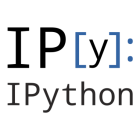
\includegraphics[width=0.4\linewidth]{ipython}
  \caption{IPython (\url{http://ipython.org}) is a rich architecture for
    interactive computing. Version 2.0 was released on April, 2014.}
  \label{fig:IPython}
\end{marginfigure} 

\begin{marginfigure}%
  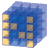
\includegraphics[width=0.4\linewidth]{numpy}
  \caption{NumPy (\url{http://www.numpy.org}) implements an N-dimensional
    array and is considered as the fundamental package for
    scientific computing with Python.}
  \label{fig:NumPy}
\end{marginfigure} 

\section{Objectives}\label{sec:objectives}
After taking this course, you should be able to:
\begin{itemize} \itemsep1pt \parskip0pt \parsep0pt
  \item use Python interactively
  \item execute a Python script at the shell prompt
  \item use Python types, expressions, and None
  \item use string literals and string type % raw and unicode strings as well?
  \item use Python statements (if...elif..else, for, pass, continue,
\ldots)
  \item understand the difference between expressions and statements
  \item understand assignment semantics
  \item write and call a simple function % (lexical scoping rule?)
  \item import and utilize a module % (Beautiful Soup?)
  \item read from and write to a text file
  \item utilize high level data structures: lists
  \item create dictionaries and complex data structures
  \item understand tuples and automatic unpacking
  \item understand the difference between mutable and immutable types
  \item write a simple class and access methods and attributes
  \item learn about how to handle and to raise exceptions
  % \item understand interpreter and compilers: CPython, PyPy, Cython
  % \item see demonstration of IDE's: IDLE, IPython, IPython
  %    Notebook, hosted environments
  % \item understand the role of package managers: easy\_install, pip
  % \item understand what NumPy does and what SciPy is (are?) 
  \item learn about resources for learning Python\footnote{tutorials,
        books, MOOC's, videos, web sites, Python Koans,
        Python Challenge, and Project Euler}
\end{itemize}

\section{Intended Audience}\label{sec:intended_audience}
This workshop is for those who have some experience in using at least
one scripting language\footnote{Stata, R, MATLAB, Perl, Ruby, emacs
lisp, bash, or PowerShell, etc.} but who do not know Python. It is
assumed that you can edit a text file using your favorite editor, and be
able to execute your script file on the command line of a shell.

\section{Environment}\label{sec:environment}
Python can be installed and used in different ways. In this workshop,
I will use IPython Notebook environment for demonstration. All the
lab PC's will have IPython Notebook installed.

If you rather use other environments, then you are welcome to bring
your own laptop computer. Free Anaconda 
distribution\footnote{Available at: 
\url{https://store.continuum.io/cshop/anaconda/}} is recomended, but
other environments (for example, command line Python and emacs editor)
are OK.

Since Python 3 is not backward compatible and not all the modules are
upgraded into Python 3, we will use Python 2 (2.7 as of writing this),
which is the default for IPython notebook in the Anaconda distribution. 

\begin{figure*}[ht]
  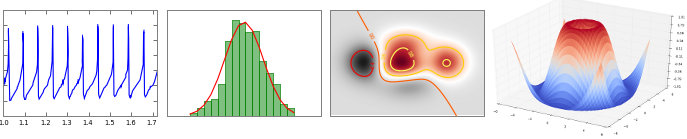
\includegraphics[width=0.8\linewidth]{matplotlib.png}%
  \caption{These plots are generated using the matplotlib module
    (\url{http://matplotlib.org}), which is a python 2D
    plotting library created by John Hunter, who unfortunately
    died of complications from cancer treatment in 2012.}%
  \label{fig:Matplotlib Plot Examples}%
\end{figure*}

\section{Location and Date}\label{sec:location_and_date}
\noindent Location: OPR Computer Lab: \#217 Wallace Hall

\noindent Date: This workshop is offerred twice. Please signup for 
one either on Thursday (Thu., May 8. 9:30 am - noon) or on Friday 
(Fri., May 9. 9:30 am - noon).

\section{Schedule}\label{sec:schedule}
\begin{table}[ht]
  \fontfamily{ppl}\selectfont
  \begin{tabular}{lll}
    \toprule
    Section & Format & Topic \\
    \midrule
    Basic Syntax & Lecture \& Quiz & Hello World to File IO \\
    Intermediate Syntax & Lecture \& Quiz & List to Exception \\
    (Optional) & Survey & Evaluation \\
    (Self-study) & Ecosystem & Demo \& Resources \\
    \bottomrule
  \end{tabular}
  \caption{Schedule. 
    We will spend most of the time going through the first two
    sections. For the third section (ecosystem and demonstration),
    a deck of slides (PDF format) and an IPython Notebook (for
    demonstration) will be provided for self-study after the workshop.}
  \label{tab:Schedule}
\end{table}

\end{document} 

